\chapter{Análisis y trazado de rectas de carga}
  Partiendo de los valores de R1 y R2 obtenidos en la seccion \ref{section:calc_r1_r2}, se busco encontrar los valores
  comerciales mas proximos a los obtenidos analiticamente, y que no afecten significativamente el punto Q. La variacion
  maxima permitida es del 10\%.
  \begin{figure}[!ht]
    \centering
    \begin{minipage}{0.7\textwidth}
      \resizebox{\textwidth}{!}{
      \begin{tikzpicture}
        \node[npn](N1) at (9.25, 5.75){} node[anchor=west] at (N1.text){$Q1$};
        \draw (7, 5) to[american resistor, l={$R_1$}] (7, 2.75);
        \draw (7, 5.75) to[capacitor, l={$C_1$}] (3, 5.75);
        \draw (7, 5.75) -- (8.41, 5.75);
        \draw (9.25, 5) to[american resistor, l={$R_E$}] (9.25, 2.75);
        \draw (3, 5.75) to[sinusoidal voltage source, l={$v_i$}] (3, 2.5);
        \draw (7, 8.75) to[american resistor, l={$R_2$}, name=R1] (7, 6.5);
        \draw (9.25, 8.77) to[american resistor, l={$R_C$}] (9.25, 6.52);
        \draw (7, 5) -| (7, 6.5);
        \draw (11, 5) to[capacitor, l={$C_E$}] (11, 2.75);
        \draw (9.25, 5) -- (11, 5);
        \draw (7, 8.75) -| (7, 9) -| (9.25, 8.77);
        \draw (11, 2.75) |- (7, 2.5) -| (7, 2.75);
        \draw (9.25, 2.75) -| (9.25, 2.5);
        \draw (3, 2.5) -- (7, 2.5);
        \draw (10.25, 6.5) to[capacitor, l={$C_2$}] (13, 6.5);
        \draw (13.75, 5.5) to[american resistor, l={$R_L$}] (13.75, 3.25);
        \draw (13.75, 6.5) -| (13.75, 5.5);
        \draw (11, 2.5) -| (13.75, 3.25);
        \node[vcc](N2) at (9.25, 9.75){} node[anchor=south] at (N2.text){$V_{cc}$};
        \draw (9.25, 9) -| (9.25, 9.75);
        \node[ground] at (9.25, 2){};
        \draw (9.25, 2.5) -| (9.25, 2);
        \draw (10.25, 6.5) -- (9.25, 6.5);
        \draw (13, 6.5) -- (13.75, 6.5);
      \end{tikzpicture}
      }
    \end{minipage}
    \begin{minipage}{0.2\textwidth}
      \centering
      \begin{align*}
        R_1 &= 10K \Omega\\
        R_2 &= 54K4 \Omega\\
        R_C &= 1K2 \Omega\\
        R_E &= 180 \Omega\\
        R_L &= 1K \Omega\\
        V_{CC} &= 12V\\
        \beta &= 484
      \end{align*}
    \end{minipage}
    \caption{Amplificador emisor común con resistencias normalizadas.}
  \end{figure}

  No logramos encontrar un conjunto de resistencias normalizadas que nos permitiesen estar dentro del margen de
  tolerancia del punto Q, asi que fijamos la $R_1$ al valor normalizado mas cercano, y jugamos con la $R_2$ para
  encontrar un serie de resistencias normalizadas. Al final, quedamos con un serie de 3K3 y 51K1. Se procede a corroborar
  si el punto Q esta dentro del 10\% del calculado con los valores analiticos de las resistencias, reemplazando su
  valor en las ecuaciones \warn ICQ REF y VCEQ REF.

  \begin{figure}[!ht]
    \centering
    \begin{minipage}{0.49\textwidth}
      \begin{align*}
        I_{CQ} &= \frac{V_{BB} - V_{BE}}{\frac{R_B}{\beta} + R_E}\\[6pt]
        I_{CQ} &= \frac{\frac{R_1}{R_1 + R_2} V_{CC} - V_{BE}}{\frac{R_1//R_2}{\beta} + R_E}\\[6pt]
        I_{CQ} &= \frac{1.86V - 1.7V}{\frac{8444.79 \Omega}{484} + 180 \Omega}\\[6pt]
        I_{CQ} &= 5.9 mA
      \end{align*}
    \end{minipage}
    \begin{minipage}{0.49\textwidth}
      \begin{align*}
        V_{CEQ} &= V_{CC} - I_{CQ} \left(R_C + R_E \right)\\[6pt]
        V_{CEQ} &= 12V - 5.9mA \left(1K2 \Omega + 180 \Omega \right)\\[6pt]
        V_{CEQ} &= 3.84V
      \end{align*}
    \end{minipage}
  \end{figure}

  Como se puede ver, el $I_{CQ}$ esta dentro del 10\% del $I_{CQ mes}$ calculado analiticamente, pero no para el
  $V_{CEQ}$. Corroborando con la simulacion en LTSpice, los valores obtenidos son parecidos, pero estos si caen dentro
  del 10\% del $I_{CQ mes}$ y $V_{CEQ mes}$ como se puede ver en la figura \ref{fig:pto_q_normalizado}. Esta diferencia
  puede ser provocada por asumir que $I_E \approx I_C$ y/o la omision de las corrientes de fuga.

  \begin{figure}[!ht]
    \centering
    \includegraphics[width=.9\textwidth]{images/pto_q_normalizado.png}
    \caption{simulacion del punto Q con resistencias normalizadas.}
    \label{fig:pto_q_normalizado}
  \end{figure}

  \section{Rectas de Carga}
    Para el trazado de las rectas de carga, se parte del analisis de la malla de salida con LKV. Para el analisis en CC,
    los capacitores pueden ser considerados como circuitos abiertos debido a que su impedancia en CC es demasiado alta.
    En la figura \ref{fig:recta_cc} puede ver el circuito resultante y el analisis con LKV.
    \begin{figure}[!ht]
      \centering
      \begin{minipage}{0.49\textwidth}
        \begin{tikzpicture}
          % Paths, nodes and wires:
          \node[npn](N1) at (1, 0){} node[anchor=west] at (N1.text){$Q1$};
          \draw (1, 1) to[american resistor, l={$R_C$}] (1, 3);
          \draw (1, -1) to[american resistor, l={$R_E$}] (1, -3);
          \node[ground] at (1, -3.5){};
          \node[vcc](N2) at (1, 3.5){} node[anchor=south] at (N2.text){$V_{CC}$};
          \draw (1, 3.5) -| (1, 3);
          \draw (1, 1) -| (1, 0.77);
          \draw (1, -0.77) -| (1, -1);
          \draw (1, -3) -| (1, -3.5);
          \draw (0.16, 0) -- (-1, -0);
          \draw (5, -0) to[american resistor, l={$R_L$}] (5, -2);
          \node[ground] at (5, -3.5){};
          \draw (5, -3.5) -- (5, -2);
          \draw (5, -0) -| (5, 1) -- (4, 1);
          \draw (2, 1) -- (1, 1);
          \draw (3, -1) |- (1, -0.77);
          \draw (3, -3) -| (3, -3.5);
          \node[ground] at (3, -3.5){};
          \node[ocirc] at (2, 1){};
          \node[ocirc] at (4, 1){};
          \node[ocirc] at (3, -1){};
          \node[ocirc] at (3, -3){};
        \end{tikzpicture}
      \end{minipage}
      \begin{minipage}{0.49\textwidth}
        \begin{align*}
          0 &= V_{CC} - V_{R_C} - v_{CE} - V_{R_E}\\[6pt]
          v_{CE} &= V_{CC} - R_C i_C - R_E i_E \qquad\to i_E \approx i_C\\[6pt]
          v_{CE} &= V_{CC} - i_C (R_C + R_E)
        \end{align*}
      \end{minipage}
      \caption{analisis para la recta de carga en CC.}
      \label{fig:recta_cc}
    \end{figure}

    Queda asi determinada la ecuacion de la recta de carga en CC para el BJT en configuracion emisor comun.

    Para el analisis de la recta de carga en CA, se procede de la misma manera. En este caso, los capacitores actuan
    como cables debido a la baja impedancia en CA. Tambien, las fuentes de alimentacion de CC actuan como
    "cortoricuitos" a masa, por lo que son reemplazadas correspondientemente. Puede revisar la figura \ref{fig:recta_ca}
    con el circuito resultante y el analisis con LKV.
    \begin{figure}[H]
      \centering
      \begin{minipage}{0.49\textwidth}
        \begin{tikzpicture}
          % Paths, nodes and wires:
          \node[npn](N1) at (1, 0){} node[anchor=west] at (N1.text){$Q1$};
          \draw (1, 1) to[american resistor, l={$R_C$}] (1, 3);
          \draw (1, -1) to[american resistor, l={$R_E$}] (1, -3);
          \node[ground] at (1, -3.5){};
          \draw (1, 3.5) -| (1, 3);
          \draw (1, 1) -| (1, 0.77);
          \draw (1, -0.77) -| (1, -1);
          \draw (1, -3) -| (1, -3.5);
          \draw (0.16, 0) -- (-1, -0);
          \draw (5, -0) to[american resistor, l={$R_L$}] (5, -2);
          \node[ground] at (5, -3.5){};
          \draw (5, -3.5) -- (5, -2);
          \draw (5, -0) -| (5, 1) -- (4, 1);
          \draw (2, 1) -- (1, 1);
          \draw (3, -1) |- (1, -0.77);
          \draw (3, -3) -| (3, -3.5);
          \node[ground] at (3, -3.5){};
          \node[ocirc] at (2, 1){};
          \node[ocirc] at (4, 1){};
          \node[ocirc] at (3, -1){};
          \node[ocirc] at (3, -3){};
          \node[ground, xscale=-1, yscale=-1] at (1, 3.5){};
          \draw (2, 1) -- (4, 1);
          \draw (3, -1) -- (3, -3);
        \end{tikzpicture}
      \end{minipage}
      \begin{minipage}{0.49\textwidth}
        \begin{align*}
          v_{CE} &= V_{CC}' - i_C (R_C//R_L),\\[6pt]
          V_{CC}' &= V_{CEQ mes} + I_{CQ mes} (R_C//R_L)
        \end{align*}
      \end{minipage}
      \caption{analisis para la recta de carga en CA.}
      \label{fig:recta_ca}
    \end{figure}

    Para trazar las rectas, podemos proceder sacando sus intersecciones en los ejes. Para CC:
    \begin{figure}[H]
      \centering
      \begin{minipage}[t]{0.49\textwidth}
        Para $V_{CE} = 0$:
        \begin{align*}
          0 =& V_{CC} - i_C(R_C + R_E)\\[6pt]
          i_C =& \frac{V_{CC}}{R_C + R_E}\\[6pt]
          i_C =& 8.695mA
        \end{align*}
      \end{minipage}
      \begin{minipage}[t]{0.49\textwidth}
        Para $i_C = 0$:
        \begin{align*}
          V_{CE} = V_{CC}\\[6pt]
          V_{CE} = 12V
        \end{align*}
      \end{minipage}
    \end{figure}

    Para CA:
    \begin{figure}[H]
      \centering
      \begin{minipage}[t]{0.49\textwidth}
        Para $V_{CE} = 0$:
        \begin{align*}
          0 =& V_{CC}' - i_C(R_C//R_L)\\[6pt]
          i_C =& \frac{V_{CEQ mes} + I_{CQ mes} (R_C//R_L)}{R_C//R_L}\\[6pt]
          i_C =& 12.94mA
        \end{align*}
      \end{minipage}
      \begin{minipage}[t]{0.49\textwidth}
        Para $i_C = 0$:
        \begin{align*}
          V_{CE} &= V_{CC}'\\[6pt]
          V_{CE} &= V_{CEQ mes} + I_{CQ mes} (R_C//R_L)\\[6pt]
          V_{CE} &= 7.05V
        \end{align*}
      \end{minipage}
    \end{figure}

    Por lo que la recta de carga nos quedaria como la de la figura \ref{fig:recta_carga}.
    \begin{figure}[!ht]
      \centering
      \begin{minipage}{0.45\textwidth}
        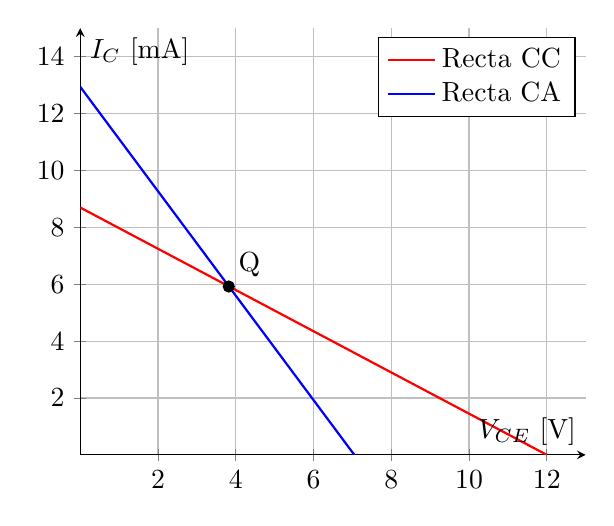
\begin{tikzpicture}
          \begin{axis}[
              axis lines=middle,
              xlabel={$V_{CE}$ [V]},
              ylabel={$I_C$ [mA]},
              xmin=0, xmax=13,
              ymin=0, ymax=15,
              grid=both,
              width=8cm,
              height=7cm,
              xtick={0,2,...,12},
              ytick={0,2,...,14},
          ]
            % Recta de CC: pasa por (0,8.695) y (12,0)
            \addplot[red, thick] coordinates {(0,8.695) (12,0)};
            \addlegendentry{Recta CC}
            % Recta de CA: pasa por (0,12.94) y (7.05,0)
            \addplot[blue, thick] coordinates {(0,12.94) (7.05,0)};
            \addlegendentry{Recta CA}
            % Punto Q
            \addplot[only marks, mark=*] coordinates {(3.82,5.92)};
            \node[above right] at (axis cs:3.82,5.92) {Q};
          \end{axis}
        \end{tikzpicture}
      \end{minipage}
      \begin{minipage}{0.54\textwidth}
        \begin{gather*}
          v_{CE_{CC}} = v_{CE_{CA}}\\[6pt]
          V_{CC} - i_C (R_C + R_E) = V_{CC}' - i_C (R_C//R_L)\\[6pt]
          i_C = \frac{V_{CC} - V_{CEQ mes} - I_{CQ mes} (R_C//R_L)}{R_C + R_E - R_C//R_L}\\[6pt]
          i_{CQ} = 5.92mA \qquad \to v_{CEQ} = 3.82V
        \end{gather*}
      \end{minipage}
      \caption{recta de carga con punto Q en interseccion.}
      \label{fig:recta_carga}
    \end{figure}

    De esta forma, corroboramos que el punto Q esta donde intersecan ambas rectas de carga. Cabe destacar que para todos
    los calculos, se utilizadon los valores calculados del punto Q con las resistencias normalizadas.
  \section{Obtención experimental de parámetros}
    \subsection{Corrientes en el divisor resistivo}
    \subsection{Verificación de resultados}

